% Note to reader: lines beginning with the '%' character are
% 'comments' to you, the human reader of this code, and are 
% ignored by the LaTeX compiler.

%%%%%%%%%%%%%%%%%%%%%%%%%%%%%%%%%%%%%%%%%%%%%%%%%%%%%%%%%%%%%%%%%%
% = Sample template for MIT Junior Lab Student Written Summaries =
% Available from 
%    http://web.mit.edu/8.13/www/Samplepaper/sample-paper.tex
%
% Last Updated July 23, 2014
%
% Adapted from the American Physical Societies REVTeK-4.1 Pages
%    at http://publish.aps.org
%
% ADVICE TO STUDENTS: Each time you write a paper, start with this
%    template and save under a new filename.  If convenient, don't
%    erase unneeded lines, just comment them out using the 
%    '%' character at the start of the line.  Often, they
%    will be useful containers for information.
%
% Using pdflatex, images must be either PNG, GIF, JPEG or PDF.
%    Turn EPS (encapsulated postscript) images to PDF using the
%    epstopdf utility on UNIX systems.
%%%%%%%%%%%%%%%%%%%%%%%%%%%%%%%%%%%%%%%%%%%%%%%%%%%%%%%%%%%%%%%%%%

%%%%%%%%%%%%%%%%%%%%%%%%%%%%%%%%%%%%%%%%%%%%%%%%%%%%%%%%%%%%%%%%%%
% = TO COMPILE THIS DOCUMENT =
%
% From the command line, it would go like this --- assuming you are
%    in the directory where the filename.tex source file and the 
%    filename.bib bibliography file are located, and that you have 
%    permission to create and write files in that directory:
%      > pdflatex filename
%      > bibtex filename
%      > pdflatex filname
%      > pdflatex filename
%    Yes, you run the command several times. The earlier runs 
%    create auxilliary files which keep track of references,
%    citations, equation and section numberring, etc. The later
%    runs combine the information in these auxilliary files with
%    your source document to create the finished product.
%
% If you are using a GUI LaTeX editor like TeXWorks, then there
%    is probably a menu bar button for pdfLaTeX and another for
%    BibTeX. Hit them in the order indicated above. There is 
%    probably also a 'TeXify' button, or something similarly named,
%    which runs all the above commands in one shot.     
%%%%%%%%%%%%%%%%%%%%%%%%%%%%%%%%%%%%%%%%%%%%%%%%%%%%%%%%%%%%%%%%%%


%%%%%%%%%%%%%%%%%%%%%%%%%%%%%%%%%%%%%%%%%%%%%%%%%%%%%%%%%%%%%%%%%%
%  = PREAMBLE =
% The preamble of a LaTeX document is the set of commands that precede
% the \begin{document} line.  It contains a \documentclass line
% to load the REVTeK-4.1 macro definitions and various \usepackage
% lines to load other macro packages.
%
% ADVICE TO STUDENTS: This preamble contains a suggested set of
%     class options to generate a ``Junior Lab'' look and feel that
%     facilitate quick review and feedback from one's peers, TAs,
%     and section instructors.  Don't make substantial changes 
%     to the style without first consulting your section 
%     instructor.
%%%%%%%%%%%%%%%%%%%%%%%%%%%%%%%%%%%%%%%%%%%%%%%%%%%%%%%%%%%%%%%%%%

%\documentclass[aps,twocolumn,secnumarabic,balancelastpage,amsmath,amssymb,nofootinbib, floatfix]{revtex4}
\documentclass[aps,twocolumn,nobalancelastpage,secnumarabic,amsmath,amssymb,nofootinbib,floatfix]{revtex4-1}

%%%%%%%%%%%%%%%%%%%%%%%%%%%%%%%%%%%%%%%%%%%%%%%%%%%%%%%%%%%%%%%%%%%
% N.B.:  Different computers have different packages installed.  
%        To compile this template in the current Athena 
%        environment, REVTeX 4.1 must be used.  To use the older
%        REVTeX 4, switch which documentclass line above is 
%        commented out above. There are ``bad'' distributions of
%        LaTeX for Windows available on the internet which may 
%        cause users to struggle unjustifiably with REVTeX 4.1.
%
%        If you are unable to compile the template at all, you
%        may need to update your LaTeX packages. (Alternatively, if 
%        your LaTeX distribution includes only the older RevTEX 4,
%        then try changing the documentclass line above. In particular,
%        this approach solves a common compilation problem for users of
%        the TeXWorks editor on Windows, which presents erroneously as a
%        error in the bibliography file.) Don't hesitate to speak 
%        with your section instructor or a TA if you're having 
%        issues getting this template to compile.
%%%%%%%%%%%%%%%%%%%%%%%%%%%%%%%%%%%%%%%%%%%%%%%%%%%%%%%%%%%%%%%%%%%

%%%%%%%%%%%%%%%%%%%%%%%%%%%%%%%%%%%%%%%%%%%%%%%%%%%%%%%%%%%%%%%%%%%
% = Explanation of documentclass options =
%
% aps, prl stand for American Physical Society and Physical 
%     Review Letters respectively.
% twocolumn permits two columns, of course.
% nobalancelastpage doesn't attempt to equalize the lengths of 
%     the two columns on the last page  as might be desired in a 
%     journal where articles follow one another closely.
% amsmath and amssymb are necessary for the subequations 
%     environment among others. These functionalities can
%     also be added use the usepackage function described below,
%     but REVTeX conveniently includes them as documentclass
%     options.
% secnumarabic identifies sections by number to aid electronic 
%     review and commentary.
% nofootinbib forces footnotes to occur on the page where they are
%      first referenced and not in the bibliography.
% floatfix attempts to help LaTeX decide where to place ``floats'',
%      like figures and plots, when it gets stuck and can't decide
%      by it's normal algorithm.
% REVTeX 4.1 is a set of macro packages designed to be used with 
%      LaTeX 2e. REVTeX is well-suited for preparing manuscripts 
%      for submission to APS journals.
%
% = Other documentclasses =
%
% The 'revtex4' and 'revtex4-1' documentclasses are somewhat 
%    specialized for making documents in the style of the APS
%    journals. For a more standard or generic looking LaTeX paper,
%    you could try any of the built-in documentclasses, in 
%    particular 'article' or 'report'. Someday, you may try to use 
%    the 'mitthesis'  documentclass available for download from the 
%    MIT Libraries. The vast majority of source code written for 
%    one documentclass should work just fine in any other, but 
%    occasional quirks arise. For example, some documentclasses 
%    disagree on whether the abstract declaration should come 
%    before or after the \begin{document} declaration.
% 
%%%%%%%%%%%%%%%%%%%%%%%%%%%%%%%%%%%%%%%%%%%%%%%%%%%%%%%%%%%%%%%%%%%

%% Now, include some packages which provide new commands that 
%% extend LaTeX's capabilities. Note that the nearly-essential
%% AMS math packages were added already as documentclass options
%% for REVTeX, but could have been added here using 
%% \usepackage{amsmath}, etc. The pacakges below are commonly 
%% useful, but there are many, many more available to solve a 
%% multitude of typesetting quandries (google your problem), 
%% and you  probably have the necesary packages installed on your
%% system already. Among the examples listed below, this sample
%% document only actually makes use of the 'graphicx', 'bm', 
%% and 'hyperref' pacakges, so the others are commented out for
%% tidyness.


\usepackage{graphicx}      % tools for importing graphics
\usepackage{lipsum}
\usepackage{float}
%\usepackage{lgrind}        % convert program code listings to a form 
                            % includable in a LaTeX document
%\usepackage{xcolor}        % produces boxes or entire pages with 
                            % colored backgrounds
%\usepackage{longtable}     % helps with long table options
%\usepackage{epsf}          % old package handles encapsulated postscript issues
\usepackage{bm}            % special bold-math package. usge: \bm{mathsymbol}
%\usepackage{asymptote}     % For typesetting of mathematical illustrations
%\usepackage{thumbpdf}
\usepackage[colorlinks=true]{hyperref}  % this package should be added after 
                                        % all others.
                                        % usage: \url{http://web.mit.edu/8.13}


%%%%%%%%%%%%%%%%%%%%%%%%%%%%%%%%%%%%%%%%%%%%%%%%%%%%%%%%%%%%%%%%%%%
% And now, begin the document...
%%%%%%%%%%%%%%%%%%%%%%%%%%%%%%%%%%%%%%%%%%%%%%%%%%%%%%%%%%%%%%%%%%%

\begin{document}
\title{Wavelength Measurement through Michelson Interferometry}
\author{Henry Shackleton}
\email{hshackle@mit.edu}
\date{\today}
\affiliation{MIT Department of Physics}


\begin{abstract}
  Using a Michelson interferometer and oscilliscope, we compare interference patterns produced by the interferometer to changes in the relative distance travelled by the two components of a split light beam before recombining. This allows us to precisely calculate the wavelength of the light beam as $620 \pm 36$ nm.
\end{abstract}

\maketitle




%%%%%%%%%%%%%%%%%%%%%%%%%%%%%%%%%%%%%%%%%%%%%%%%%%%%%%%%%%%%%%%%%%

A Michelson interferometer is a device where a beam of light can be split in two perpendicular directions, recombined, and then measured via a photodetector. By varying the length that one of the two split beams travels, one can produce interference patterns that can be detected by the photodetector. This setup was originally devised by Michelson in 1881 to test whether light propegated through an "aether," which could cause the light to travel more slowly in one direction than the other, thereby producing an interference pattern \cite{michelson}. His experiment, along with others of the time period, eventually showed that light travelled at the same speed irrespective of direction. However, the  Michelson interferemoter has proven to be useful for other measurements, such as the one described here.
  \\
  As variations in length will be the predominant contributor to interference patterns, by varying the length precisely via a PZT (Piezoelectric Transducer) we can detect with high precision the length changes that correspond to various interference patterns. This allows us to calculate the wavelength of the beam of light under study. Through this procedure, we are able to calculate the wavelength of the light beam used as $620 \pm 36$ nm.
  \\
  \section{Theory}
  The primary theoretical background necessary for this experiment is understanding the process of combining two light beams. Although a full theory of light requires a description of the underlying quantum phenomena, for the purposes of light interference, we can treat light as a wave, described by some amplitude $E_1$ , a phase $\phi_1$, and an angular frequency $\omega$.
  \begin{equation}
    E(t) = E_1 e^{i(\phi_1 - \omega t)}
  \end{equation}
  The variable $t$ denotes the time of interest. Although the full equation of a light wave will have some position dependence, for the purposes of this experiment, we will only be concerned with the time dependence of the wave at a fixed position. Combining two beams of light consists of superimposing the wave equations describing them. To understand this mathematically, let us introduce a second equation to describe the second beam of light, with the same frequency $\omega$ but with a different amplitude $E_2$ and phase $\phi_2$.
  %\begin{equation}
  %  \tilde{E}(t) = E_2 e^{i(\phi_2 - \omega t)}
  %\end{equation}
  Adding these two equations together gives
  \begin{equation}
    E_T =  E_1 e^{i(\phi_1 - \omega t)}+  E_2 e^{i(\phi_2 - \omega t)}
  \end{equation}
  The form of this combined wave depends on the difference between $\phi_1$ and $\phi_2$. If $\phi_1$ and $\phi_2$ differ by a complete phase, $\phi_1 - \phi_2 = 2\pi n $ for some integer $n$, then the equation reduces to
  \begin{equation}
    E_T = (E_1 + E_2) e^{-i\omega t}
  \end{equation}
  This is known as \textit{constructive interference} - the amplitudes of the two waves add to each other. If $\phi_1$ and $\phi_2$ differ by half a phase, $\phi_1 - \phi_2 = (2n + 1)\pi$, then the equation instead reduces to
  \begin{equation}
    E_T = (E_1 - E_2) e^{i \omega t}
  \end{equation}
  This is called \textit{destructive interference}, as the amplitude of the two waves detract from each other. In the case of equal amplitude waves, $E_1 = E_2$, destructive interference results in a perfect cancellation of the two waves. An example of this is shown in \ref{fig:super}.
  \begin{figure}
    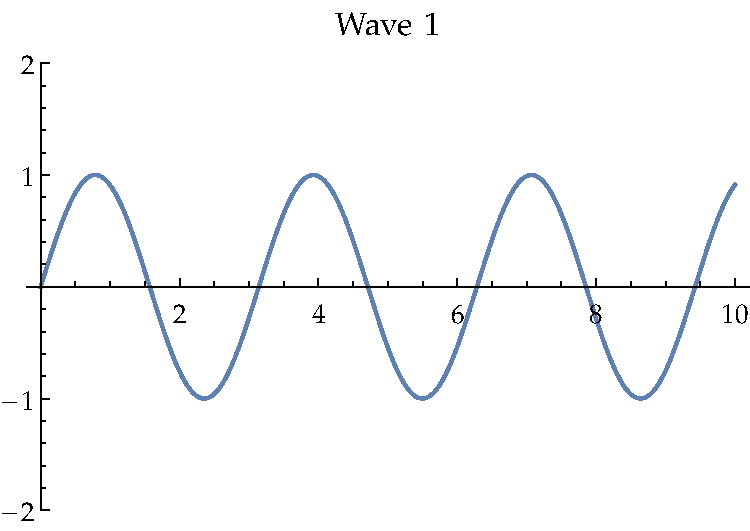
\includegraphics[width=0.4\textwidth]{sin1.pdf}
    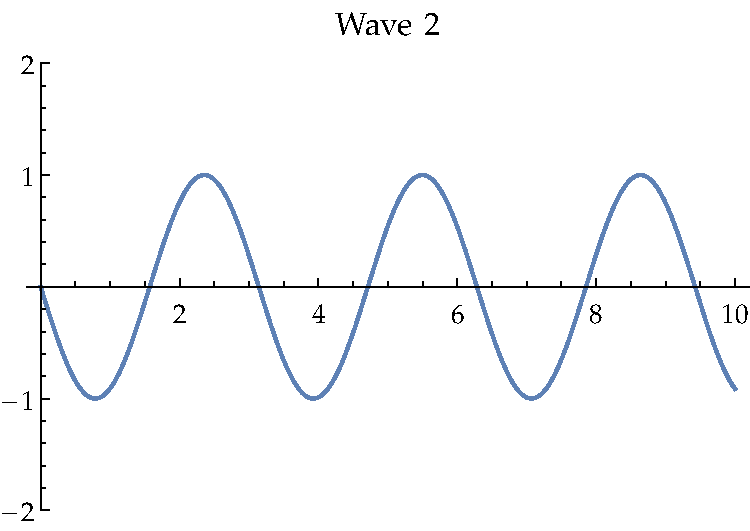
\includegraphics[width=0.4\textwidth]{shifted.pdf}
    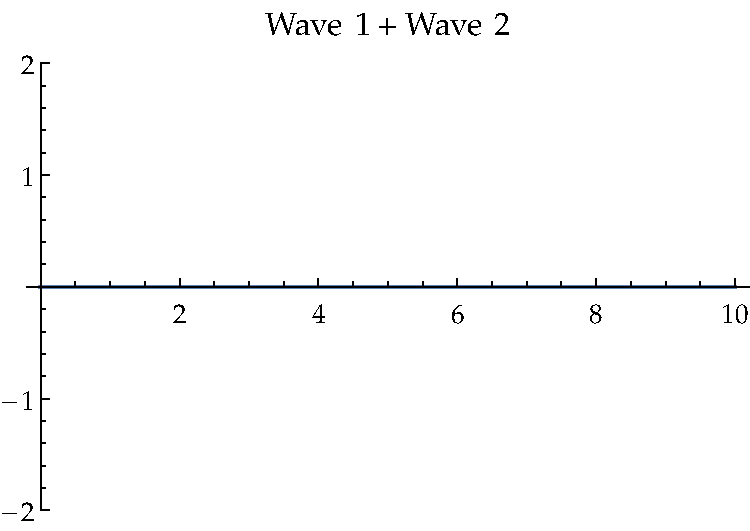
\includegraphics[width=0.4\textwidth]{destructive.pdf}
    \caption{An example of destructive interference with two waves of equal amplitude. When two waves with a relative phase offset of $(2n+1)\pi$ are superimposed, the two waves are cancelled out.}
    \label{fig:super}
  \end{figure}
  \\
  Our photodetector does not measure the wave itself, but rather the \textit{intensity}, $I$, of the wave. The intensity of a wave is given by taking the square of the wave and averaging it over time, which in the case of the two superimposed waves, gives
  \begin{equation}
    I \propto E_1^2 + E_2^2 + 2E_1 E_2 \cos(\phi_1 - \phi_2)
  \end{equation}
  Constructive and destructive interference affect the intensity - with constructive interference, $\cos(\phi_1 - \phi_2) = 1$, and with destructive interference, $\cos(\phi_1 - \phi_2) = -1$.
  \\
  In our setup, a beam splitter separates a light beam into two beams of equal amplitude, and then the two beams are combined at a later stage. A phase difference is induced by the different lengths that the two beams travel. The correspondence between the phase difference and length difference is determined by the wavelength $\lambda$ of the beam. If one beam travels a distance of $2l_1$ before recombining, and the second beam travels a distance of $2l_2$, the phase difference is given as
  \begin{equation}
    \phi_2 - \phi_1 = \frac{4 \pi}{\lambda} \left(l_2 - l_2\right)
  \end{equation}
  %Ideally, this would result in perfect cancellation in the case of destructive interference, and a doubling of the intensity in the case of constructive interference. A number of factors, such as the light not splitting into beams of equal amplitude, or the two beams not recombining at the same location, can cause deviations from this ideal scenario. These deviations can be made qualitative by the interferometric visibilitly $\mathcal{V}$, 
  %\begin{equation}
  %  \mathcal{V} = \frac{I_{max} - I_{min}}{I_{max} + I_{min}}
  %\end{equation}
  %Where $I_{max}$ and $I_{min}$ represent the maximum and minimum intensities measured, respectively. In an ideal setting, $I_{min} = 0$ and $\mathcal{V} = 1$ - deviations from this will cause the visibility to dip below $1$.

  \section{Experimental Setup}
  The source of our light beam will be an orange laser, which emits a constant light source of a certain wavelength. A beam splitter is positioned along the trajectory of the beam at a 45 degree angle, which splits the beam into two beams of approximately equal amplitude, each travelling perpendicular to the other. One of the beams travels a length $l_2$, is reflected by a mirror, and is sent back to be detected by a photodetector. The other beam travels a length $l_1$ and reaches a mirror connected to a PZT (piezoelectric transducer). The PZT is connected to a function generator, which supplies the PZT with a varying voltage in the form of a triangle waveform with a peak-to-peak voltage of 10V and a frequency of 10Hz. The PZT translates these supplied voltages to spatial translations along the length of $l_1$. The PZT used in this experiment has a response of $44.6 \pm 2.6$ $nm/V$. As the voltage varies, the length that the beam of light travels to reach the mirror varies from $l_1 + \Delta$ to $l_1 - \Delta$, where $\Delta$ is some small displacement induced by the PZT. The function generator applied to the PZT is additionally connected to an oscilliscope, which allows us to read off the voltage being supplied to the PZT, and therefore the difference in length in the trajectory of the light beam.
  \\
  \begin{figure}[t]
    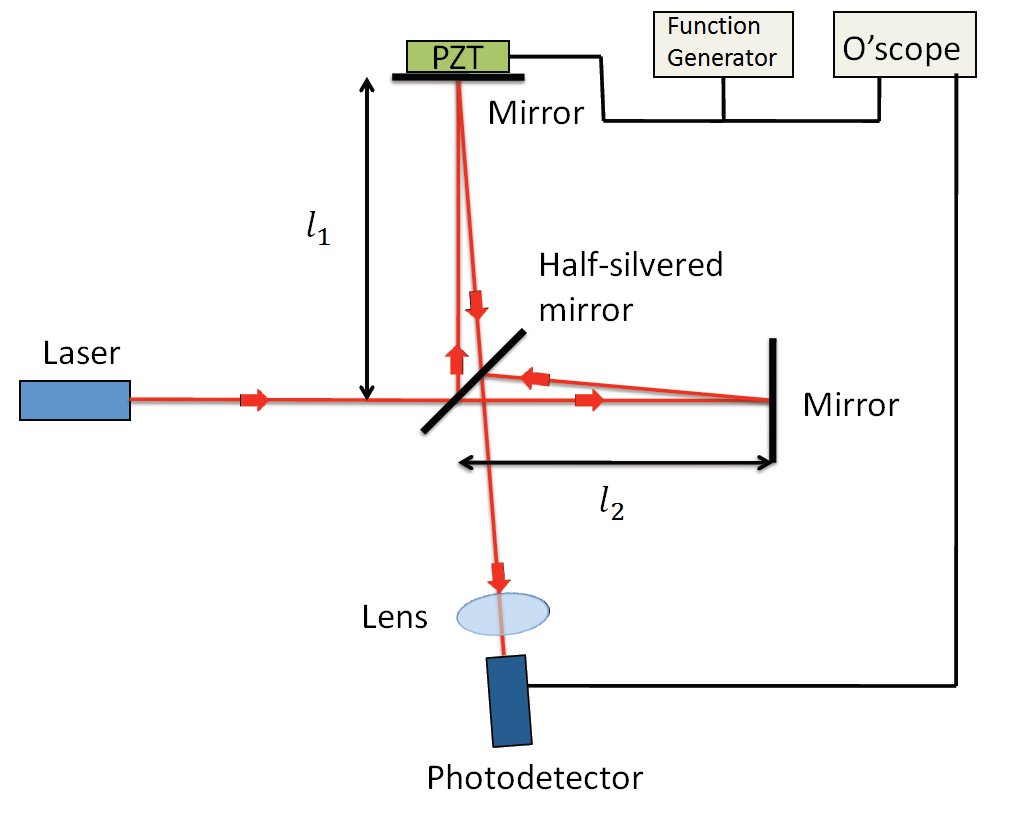
\includegraphics[width=0.4\textwidth]{setup.png}
    \caption{A block diagram of our experimental setup, with lengths $l_1$ and $l_2$ indicating the distance travelled by each of the two light beams. \cite{michelsonmanual}}
  \end{figure}
  Both light beams are reflected by the mirrors, and recombined at a photodetector, which measures the intensity of the beam. A crucial calibration step in this experiment is positioning the two mirrors so that the two beam align perfectly on the photodetector. Any deviations from this will reduce the signal measured. The photodetector is connected to the oscilliscope previously mentioned. This allows us to simultaneously measure the voltage supplied to the PZT - and in virtue of that, the displacement of the mirror attached to it - and the intensity of the resulting beam.
  \section{Data Analysis}
    Figure \ref{fig:waveform} gives an example form of a signal seen on our oscilliscope. At every maximum in the orange line - representing the intensity of the measured beam - complete constructive interference is taking place between the two beams. At every minimum, complete destructive interference is taking place. This change in interference is induced by the change in relative phase between the two beams, which is caused by the differences in length produced by the PZT.
   \begin{figure}[t]
    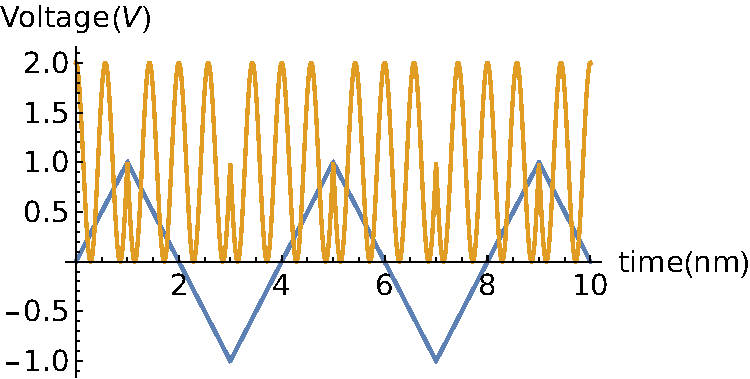
\includegraphics[width=0.4\textwidth]{waveform.pdf}
    \caption{An example reading of the oscilliscope, generated in Wolfram Mathematica. The blue line corresponds to the signal from the function generator, and the orange line corresponds to the intensity measured by the photodetector. A linear change in voltage corresponds to a periodic chance in intensity, with cusps at the points where the voltage switches direction.}
    \label{fig:waveform}
    \end{figure}
    The change from one maxima to another, or the change from one minima to another, corresponds to a change in the length travelled by one of the beams equal to the wavelength. This is a direct consequence of equation (6). Therefore, calculating the voltage differences supplied to the PZT across maxima and minima, and then determining the displacement length corresponding to that voltage. we are able to determine the wavelength of the laser beam.
    \\
    Over the course of taking measurements of this voltage difference, we will accumulate a distribution of values. Using this distribution, we can calculate a mean, along with some statistical uncertainty for this value. Using this value, we can use the response value of the PZT, with its associated uncertainty, to come to final conclusion and uncertainty of our laser's wavelength.
    \begin{figure}[h]
      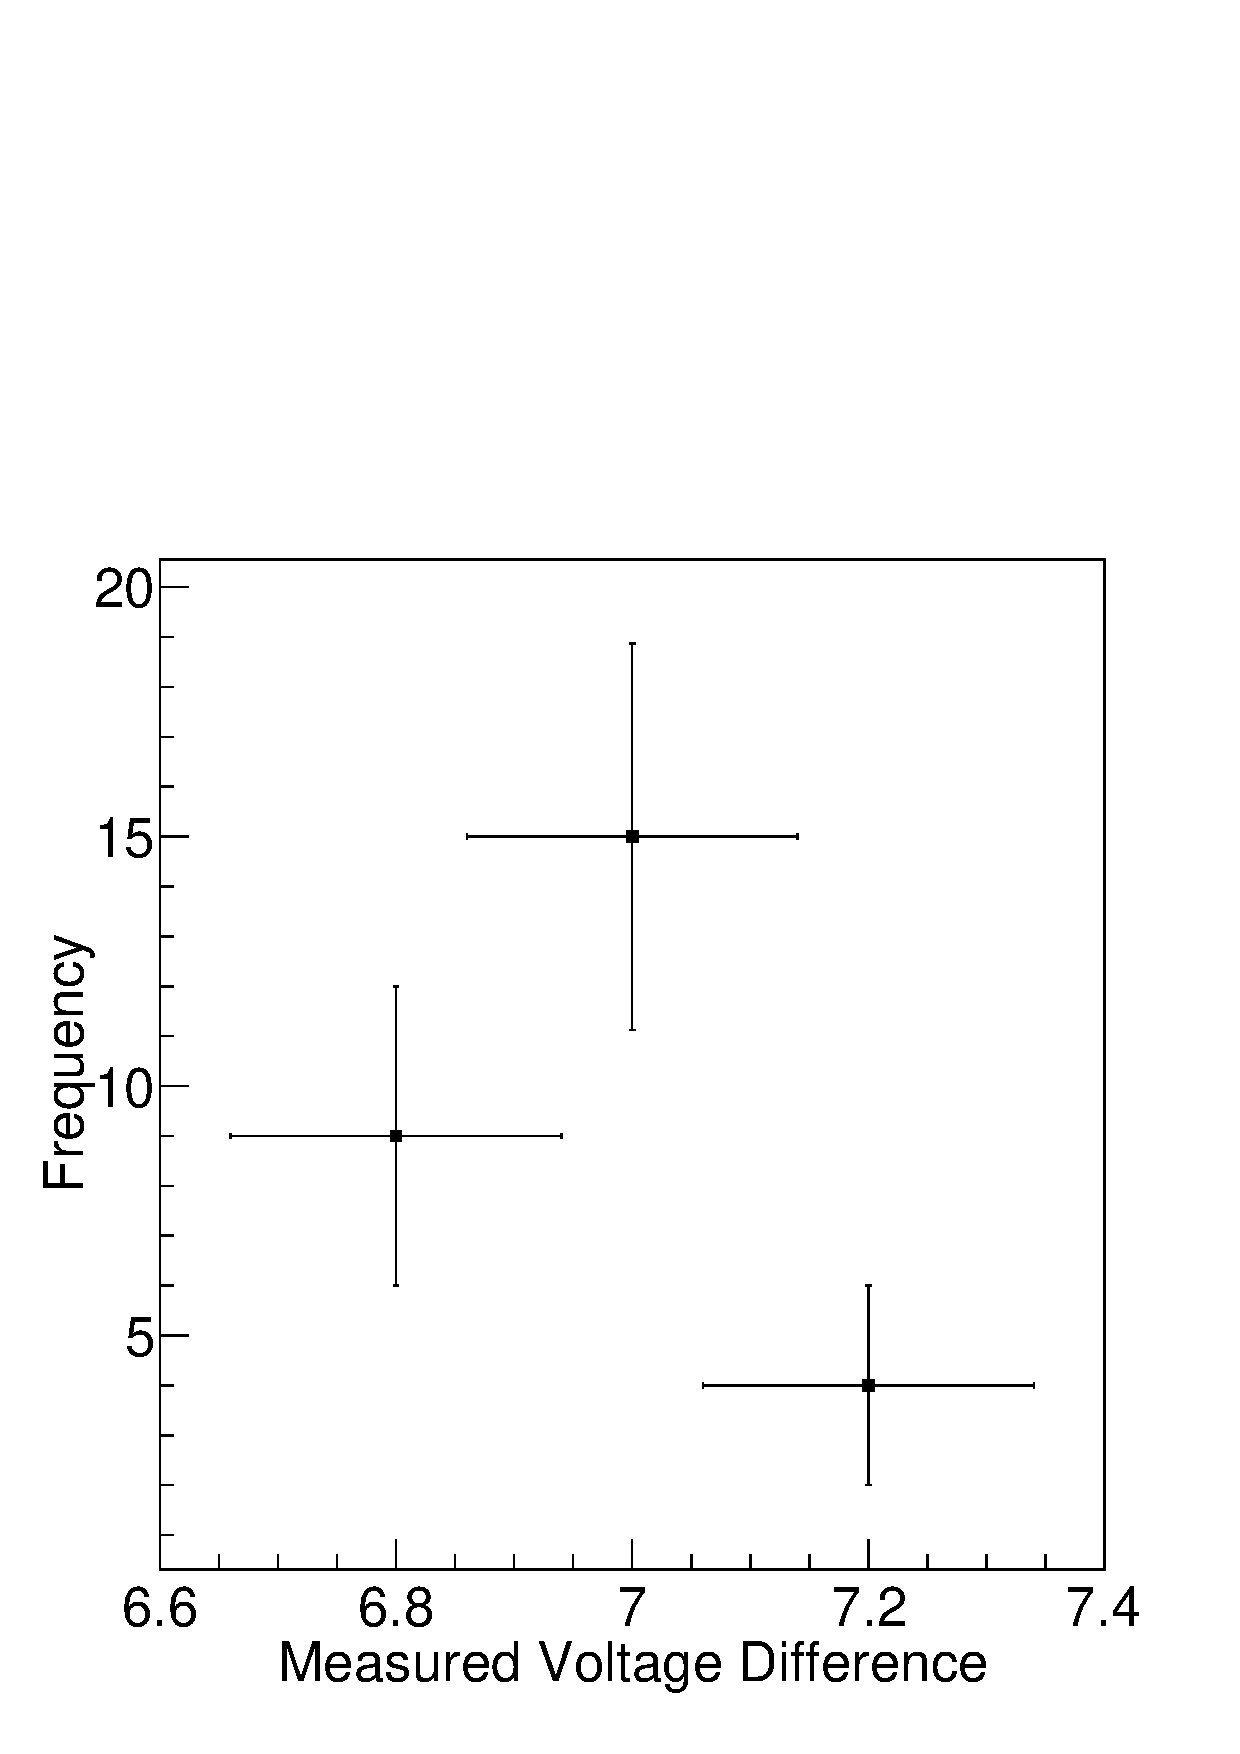
\includegraphics[width=0.45\textwidth]{graph_helvetica.pdf}
      \caption{A distribution of the measured voltage differences between minima and maxima of interference peaks, with associated uncertainties for the frequency counts.}
      \label{fig:graph}
    \end{figure}
    \\
    In our experiment, we conducted 29 measurements of the voltage difference across maxima and minima, represented visually in \ref{fig:graph}. Each individual voltage measurement has associated uncertainty of $\pm 0.1$ V due to the oscilliscope measurements being taken from reading off the values by eye. As two measurements are necessary to determine a voltage difference, this results in a total uncertainty of $\pm 0.14$ V. Taking the average of these measurements and calculating the uncertainty associated with this average, we arrive at an average voltage difference of $6.96 \pm .14 $ V. As the distribution of values was closely-packed, averaging over them only gives an additional uncertainty of $\pm 0.02$ V, which does not noticeably modify our initial uncertainty of $\pm 0.14$. Converting this average voltage into length displacement, we conclude that the predicted wavelength of the laser is $620 \pm 38$ nm. This is within the visible spectrum, and roughly corresponds with the observed colour of the laser. Because of this, we can conclude that Michelson interferometers provide a method of detecting wavelengths of supplied light sources to within a reasonable degree of accuracy.
    
    \begin{figure}[h]
      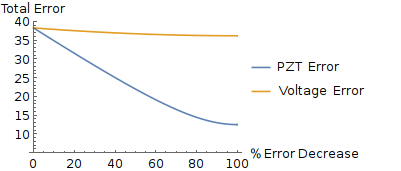
\includegraphics[width=0.5\textwidth]{error.png}
      \caption{A graph showing the effects on the total uncertainty that a decrease in uncertainty in either the PZT or voltage uncertainties would have, relative to the uncertainty values in this experiment. A decrease in the PZT uncertainty causes a more drastic change in the overall uncertainty.}
      \label{fig:error}
    \end{figure}
    By looking at our error propegation further, one can see that our PZT response of $44.6 \pm 2.6$ $nm/V$ is the single largest contributor of uncertainty in our experiment. As shown visually in \ref{fig:error}, a decrease in PZT uncertainty causes a larger change in the overall uncertainty than a decrease in our uncertainty in our voltage measurement. As such, in future iterations of this experiment, an effective method of decreasing uncertainty would be to acquire a PZT with a smaller uncertainty range.
    \section{Conclusion}
    Michelson interferometers allow one to detect interference patterns created through the relative phase difference of two laser beams. By varying this phase in a controlled manner and comparing this to the interference patterns recorded, we are able to determine the wavelength of the source laser with an uncertainty of less than 50 nanometers. 
    \begin{acknowledgements}
    I would like to thank my 8.13 lab partner, Adin Hrnjic, for assisting with this experiment as well as providing invaluable guidance through the analysis of our data. Additionally, I would like to thank Rudy Garcia for additional guidance throughout the analysis of our data.
  \end{acknowledgements}

  \bibliography{michelson-paper}

\end{document}
